\chapter{Interfaces}
\label{ch:Interfaces}
The interfaces act as the main vessel for keeping track of all connections throughout the \textit{Swing}; hence, they should be correctly followed.
\Cref{sec:N2Chart} further elaborates upon the interfaces of all the (sub)systems of the eVTOL, which helps the understanding of all parameter correlations.
Subsequently, the hardware diagram in \Cref{sec:HardwareDiagram} provides the extensive interface picture from within the vehicle, broadening the scope further than only the autonomous system.
This will be further strengthened by the Data Handling Diagram in \Cref{sec:data_handling}, completing the interface perspective.

\section{N2 Chart}
\label{sec:N2Chart}
The N2 chart can be seen as the main tool for understanding the relations between interfaces of all relevant (sub)systems.
The green boxes in \Cref{fig:N2chart} represent the main subsystems of the \textit{Swing eVTOL}.
Each is connected to its distinctive in- and outputs, following a clockwise motion.
For instance, when looking at Aerodynamics and Flight Performance, the inputs for Flight Performance are aerodynamic coefficients and wing planform.
It will then output the cruise and stall speed, climb rate, climb angle, and flight envelope.
In return, these will act as inputs for the Aerodynamics system, which will then deliver new values for the aerodynamic coefficients and wing planform.
Therefore, the N2 Chart  showcased in \Cref{fig:N2chart} provides a clear overview of all in- and outputs between (sub)systems.

\begin{figure}[H]
    \centering
    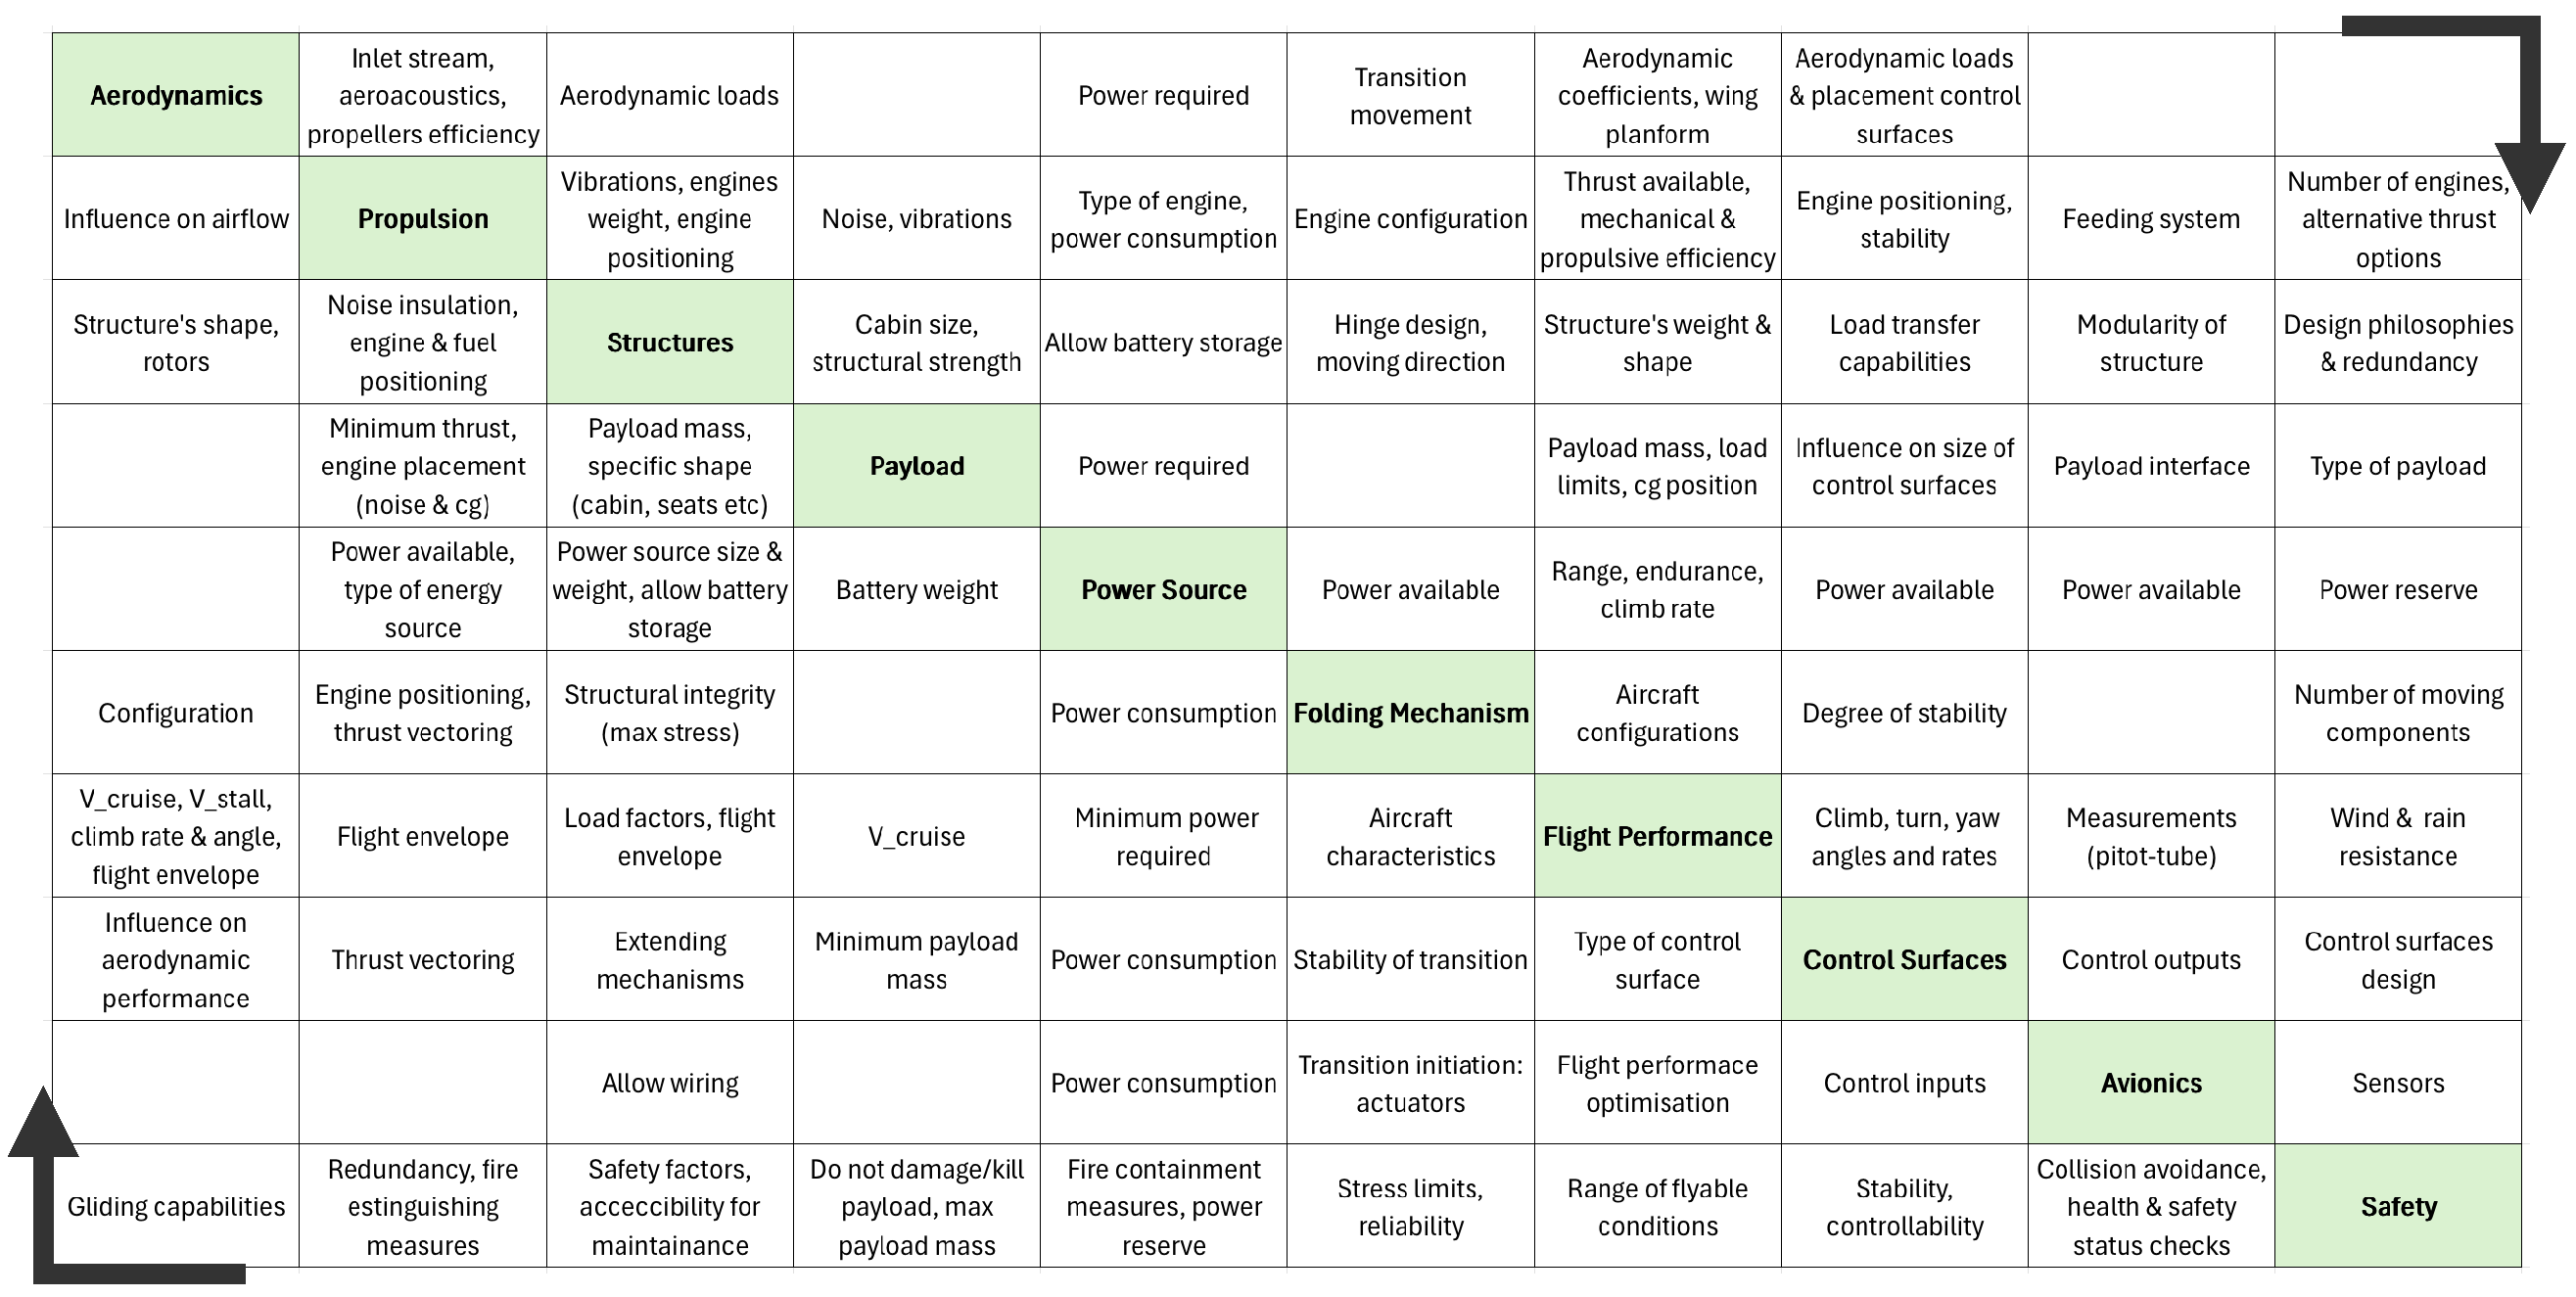
\includegraphics[width=0.9\linewidth]{figures/New N2-chart}
    \label{fig:N2chart}
    \caption{N2 chart of (sub)systems}
\end{figure}

\section{Hardware Diagram}
\label{sec:HardwareDiagram}
To clearly visualise the hardware components of the \textit{Swing eVTOL}, \Cref{fig:hwdiag} accompanied by an acronym list in \Cref{tab:hwdiagacronyms} fully show it.
The main hardware components or groups are distinguished by white boxes, the actuation and sensor groups, given their diversity in composing parts, are instead grouped into the red and yellow frames respectively.
The sections of the diagram relative to the ground segment can be deduced by their parallelogram shapes.

\begin{table}[H]
\centering
\caption{List of acronyms with reference to \Cref{fig:hwdiag}}
\label{tab:hwdiagacronyms}
\begin{tabular}{clcl}
\textbf{FCC} & Flight Control Computer    & \textbf{GNSS} & Global Navigation Satellite System \\
\textbf{VMS} & Vehicle Monitoring Sensors & \textbf{IMU}  & Inertial Measurement Unit          \\
\textbf{BMS} & Battery Management System  & \textbf{PDU}  & Power Distribution Unit           
\end{tabular}
\end{table}

\begin{figure}[H]
    \centering
    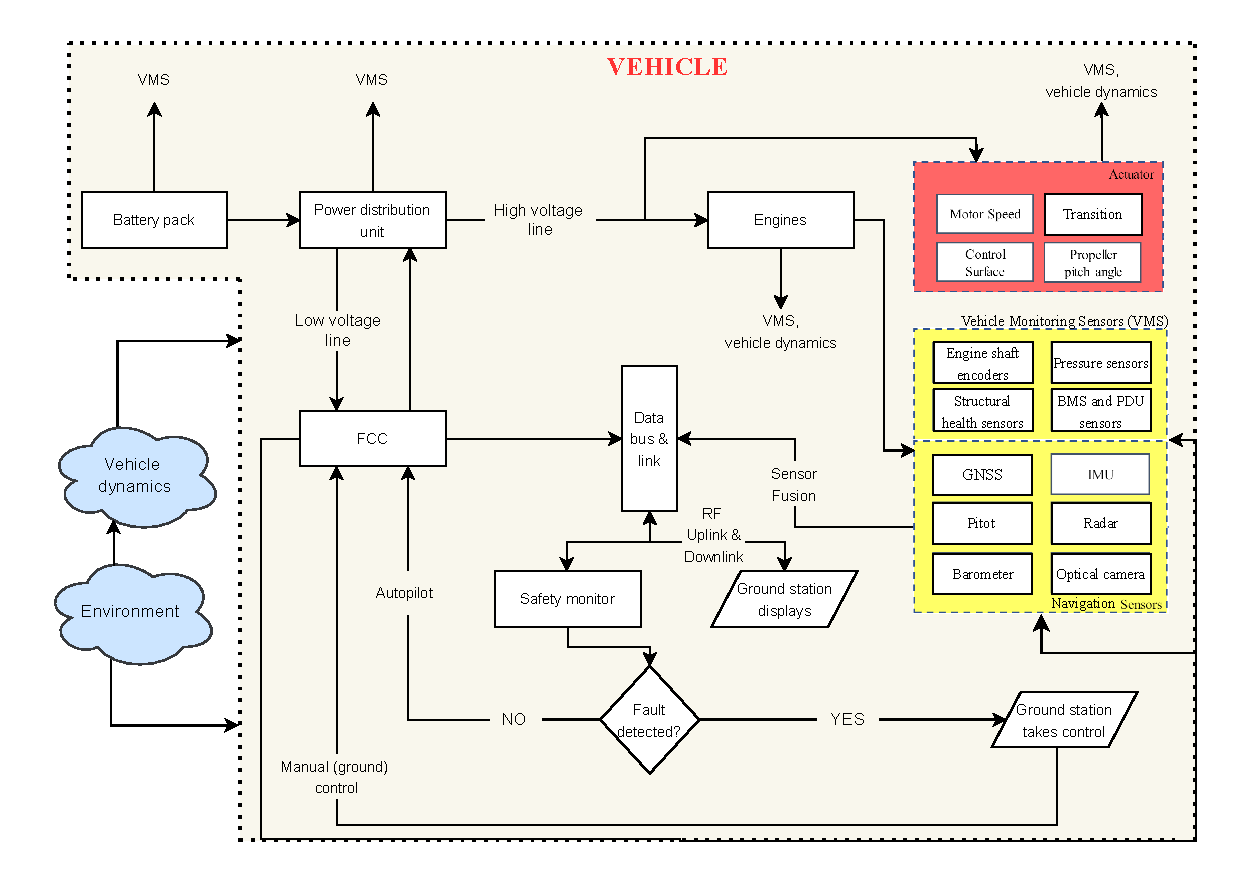
\includegraphics[width=\linewidth]{figures/HWdiagramUPDATED}
    \caption{H/W diagram}
    \label{fig:hwdiag}
\end{figure}


\subsection{Diagram Flow Discussion}
The PDU manages the battery energy, which appropriately distributes it to the components of interest.
It follows orders from the FCC, which is the \enquote*{brain} of the vehicle, where the main navigation, control and vehicle-handling software is located and executed.
The orders outputted are based on the current power requirements and vehicle state.
Two power lines can be distinguished coming from the PDU due to the substantially different power ($\text{power}=\text{voltage}\times \text{current}$) requirements: high- and low-voltage lines.
The high-voltage line powers the actuators and engines according to the thrust and attitude settings dictated by the FCC. 
Whereas the low-voltage line is connected directly to the FCC, which distributes the energy to all the low-power components in the vehicle, such as sensors.

The state of the aircraft is constantly monitored by a set of sensors measuring the state of the vehicle, speed, and attitude.
The actuators change the aircraft’s state and configuration in hover or cruise.
Sensor data is processed via sensor fusion algorithms before being fed to the FCC for analysis.
A safety monitoring board is connected to the data bus, and if a critical functional flaw is detected, action is taken.
It is finally important to underline the iterative nature of this diagram: in every cycle the vehicle responds to the environment and its dynamics via the actuators, which in turn leads to a change in vehicle dynamics, thus yielding a new set of commands.
This is represented by those arrows ending on and coming from the dotted line, figuratively representing the vehicle update cycle iteration.


\subsection{Sensors}
A list of the sensors used is provided below, along with a rationale for each component (the unit numbers will be established in later design phases):
\begin{itemize}
    \item \textbf{Engine shaft encoders:} allowing for real-time determination of the RPMs per engine and accurate thrust adjustments.
    \item \textbf{Pressure sensors:} allowing to measure and monitor, for instance, hydraulic pressures, pressure differential across the cabin, etc.
    \item \textbf{Structural health sensors:} group of sensors delegated to perform damage detection, event and monitoring (i.e.\ Mechanical Impact Diagnosis using passive piezoelectric sensors, impact damage diagnosis)~\cite{hwdiagHEALTH}.
    \item \textbf{BMS} and \textbf{PDU sensors:} allowing for constant monitoring of battery and power lines health.
    \item \textbf{GNSS:} \enquote*{providing positioning, navigation, and timing using navigational satellites from other networks beyond the GPS system} \cite{gpsgov}
    \item \textbf{IMU:} determines the specific angular rate, body orientation and force acting on it, using a combination of accelerometers, gyroscopes and magnetometers.
    \item \textbf{Pitot tube:} enables computation of the vehicle’s speed.
    \item \textbf{Radar:} allows for automated collision avoidance procedures.
    \item \textbf{Barometer:} allows for the vehicle’s altitude computation.
    \item \textbf{Optical camera:} can transmit real-time footage back to the ground and allow for the implementation of computer vision algorithms.
\end{itemize}

\subsection{Actuators}
A list of the main actuators used is provided below, along with a rationale for each component (the unit numbers will be established in later design phases):
\begin{itemize}
    \item Control of \textbf{motor speed} and \textbf{control surfaces deflection angles} directly influences the vehicle’s state, adapting it to its current settings.
    \item Actuation of \textbf{transition} mechanisms regulates the configuration change.
    \item Adjusting the \textbf{RPM} of the propellers mainly allows one to optimise the aircraft settings based on its current configuration.
\end{itemize}


\section{Data Handling Diagram}
\label{sec:data_handling}
Finally, the data handling flow diagram shows the communication and data management within the UAM’s hardware. Three external data sources are present in the process.
Data is collected through telecommunication from ground control and other vehicles, as well as measurements of the digital and analogue sensors.
After analogue filtering and converting, the necessary signals are converted to digital signals, and two possibilities arise.
The data can either flow directly to the Central Processing Unit (CPU), through the serial bus or be fed to a microcontroller.
If the second option is used, one directional communication can be achieved, and the CPU can also send data to the sensor, adding the possibility of measurement range and offset adjustments.
The bus further ensures the communication link with the actuator controllers.
Finally, the transmitter antenna closes the communication loop with the ground control. The described data handling diagram is shown in\Cref{fig:data_handling_diagram}
\begin{figure}[H]
    \centering
    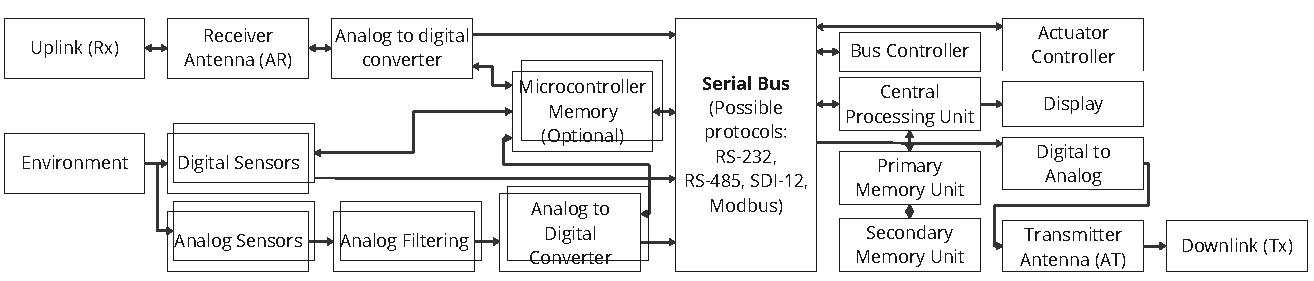
\includegraphics[width=\linewidth]{figures/Interfaces/data_handling_diagram}
    \caption{Data handling flow diagram}
    \label{fig:data_handling_diagram}
\end{figure}
